\documentclass[a4paper]{exam}

\usepackage{geometry}
\usepackage{graphicx}
\usepackage{hyperref}
\usepackage{mathtools}
\usepackage{titling}

\printanswers

\title{Weekly Challenge 06: Divide and Conquer\\CS 412 Algorithms: Design and Analysis}
\author{q1-team-2}  % <==== replace with your team name for grading
\date{Habib University | Spring 2023}

\runningheader{CS 412: Algorithms}{WC06: Divide and Conquer}{\theauthor}
\runningheadrule
\runningfootrule
\runningfooter{}{Page \thepage\ of \numpages}{}

\qformat{{\large\bf \thequestion. \thequestiontitle}\hfill}
\boxedpoints

\begin{document}
\maketitle

\begin{questions}


	\titledquestion{k-th largest}

	We want to explore the efficiency of different approaches to solve the following problem.

	\begin{tabular}{ll}
		\textbf{Input}:  & A sequence, $A$, of $n$ numbers $\langle a_1, a_2, a_3, \ldots, a_n \rangle$ in arbitrary order   \\
		                 & A number, $k$ where $1 \leq k \leq n$                                                             \\
		\textbf{Output}: & $a_i$ where the sequence $\langle a_j \mid a_j \geq a_i, i\neq j \rangle$ contains $k-1$ elements
	\end{tabular}
	\smallskip

	\subsection*{Tasks}
	\begin{description}
		\item[Divide and Conquer] Use the strategy given in Section 2.4 of Dasgupta et al. to implement the \textit{select} function in the accompanying file, \texttt{test\_select.py}.
		\item[Correctness] Run \texttt{pytest} locally to check your implementation.
		\item[Sorting] In the same file, implement the \textit{select\_sort} function using the strategy used in the \textit{test\_select} function.
		\item[Compare] Plot the run time of your algorithms in a single diagram over a wide range of $n$. Make sure that each plot is clearly labeled, or the diagram contains a clearly visible legend. Make sure that the axis limits are set such that the plots are clearly visible and occupy a large portion of the diagram. Include separate diagrams over different axis ranges for greater clarity if necessary.
		\item[Submit] Include the diagram in your solution below.
		\item[Comment] Include below any observations or comments that you find significant.
		\item[Share] Share your diagram as a comment on the \href{https://web.yammer.com/main/org/habib.edu.pk/threads/eyJfdHlwZSI6IlRocmVhZCIsImlkIjoiMjEzNDMyMjU5OTgxMzEyMCJ9}{WC06 post} in the course group.
		\item[Attribution] Adherence to the usual attribution practices is expected. Make sure to cite any external sources.
	\end{description}

	\begin{solution}
		% Enter your solution here.
    \\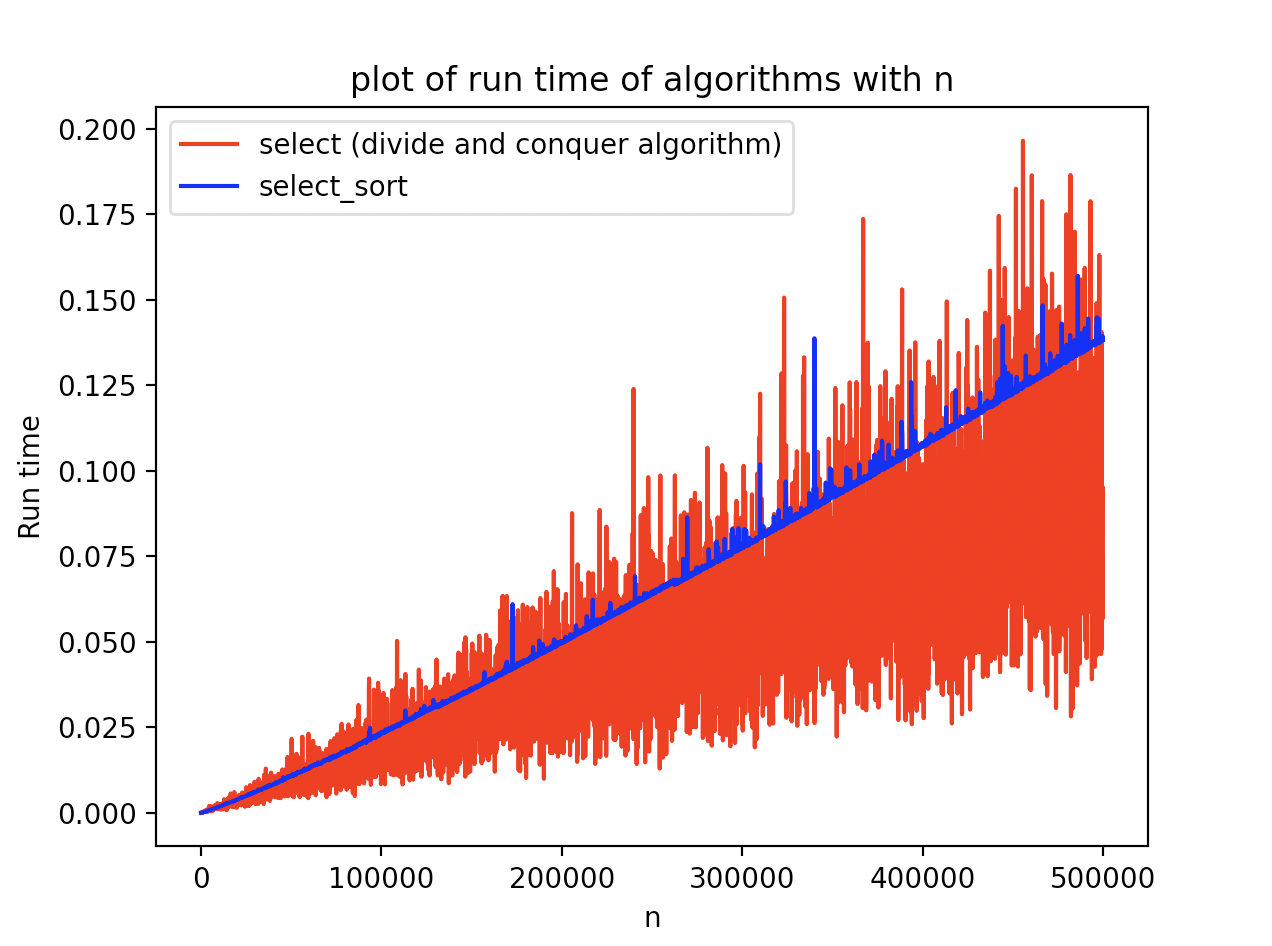
\includegraphics[scale = 0.5]{plot(100,500000,100).png}
    We can see that the plot for select (divide and conquer algorithm) fluctuates a lot where as the plot for selete\_sort is much more stable.
    We believe this is becuase select is a randomized algorithm, so for good values of v (closer to median) the time taken is smaller but for larger values its much greater.
    So for good values of v the time taken by select is much lower than the time taken by select\_sort but for bad values its greater.
	\end{solution}

\end{questions}

\end{document}
